\chapter{Online Adaptation}
\label{chap:adaptation}
%\url{https://github.com/clab/fast_align}
In this chapter, we experiment with online adaptation of the proposed enhanced ASR pipeline.

We assume that many ASR errors are systematic and highly dependent on the particular speaker, for example, due to his/her mother tongue. We expect that some of these errors can be identified and corrected in the ASR phoneme-to-grapheme translation model. We plan to identify these corrections and extract simple speaker-specific rules. %These rewriting rules would be applied before feeding them into the ASR/SLT translation model in the pipeline.

This chapter is organized as follows: in \cref{oeasr:model} we propose online adaptation and incorporate it into the proposed ASR/SLT pipeline. In \cref{oeasr:experiments}, we experiment with the online adaptation. Finally, in \cref{oeasr:conclusion} we conclude the chapter.

\section{Enhanced ASR/SLT Pipeline with Online Adaptation}
\label{oeasr:model}
We propose the enhanced ASR pipeline with online adaptation as follows: the acoustic model outputs the phoneme transcripts. The phoneme transcripts are adapted using the Online Adaptation model. The adapted output (still in phonemes) is fed into the phoneme-to-grapheme translation model (note, under the term translation we mean both the monolingual --- phonemes to graphemes in the same language --- and translation from source language phonemes to target language graphemes). The translation model translates the phoneme input into graphemes using beam search. The model outputs the best translation candidate from the beam as a translation of the whole ASR pipeline. All beam translations are passed through the \texttt{phonemizer}, and the online adaptation model learns new rules from the transcripts.

In the case of the SLT pipeline, two parallel phoneme-to-grapheme translation models are needed: the ASR and the SLT. The ASR translation model would be used for obtaining ``training data'' for the online adaptation model.

The schema of the proposed enhanced ASR pipeline with online adaptation is in \cref{fig:online_easr}.

\begin{figure}[t]
    \centering
    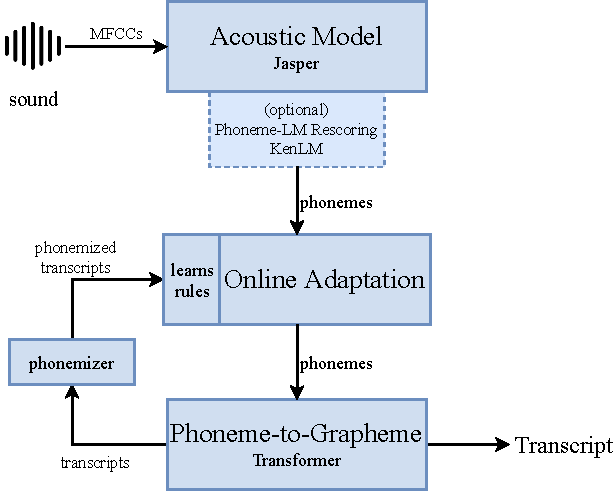
\includegraphics[width=.9\textwidth]{img/online_easr}
    \caption{Enhanced ASR pipeline with online adaptation.}
    \label{fig:online_easr}
\end{figure} 


\subsection{Online Adaptation Model}
We seek a method that would be capable of quick, on-the-fly adaptation as a speaker talks. The apparent requirement of such online adaptation model is that it must be able to learn quickly. Hence, we rule out neural networks as they require a higher volume of training data. Short of such data, the neural networks tend to over-fit the examples. 

Therefore, we decided on the rule-based model. We take our inspiration in the work we previously reviewed for phoneme-to-grapheme models (see \cref{easr:rel_asr}). More precisely, the work of \perscite{horndasch2006phoneme}. Their main objective is to find appropriate orthographic representations for phoneme strings. Our use case differs as we seek phoneme-to-phoneme mapping correcting errors instead of phoneme-to-grapheme mapping. Using an expectation-maximization algorithm \parcite{dempster1977maximum}, we seek the best ``correct-to-incorrect'' phoneme alignment (in their setup, they are looking for best phoneme-to-grapheme alignment). In the second step, we cluster neighboring symbols together to account for the insertions (i.e., to remove ``$\epsilon$ to phoneme'' rules). Finally, $n$-gram probabilities of symbol pairs are learned. During the inference, the input string is split into individual phoneme symbols. For each symbol are generated all possible symbol pairs. According to the beam width, the best sequences are taken. 

\paragraph{Model Training}
As already described, we learn the phoneme rewrite rules from aligned ``incorrect-to-correct'' phoneme transcriptions. To align these transcriptions, we utilize the expectation-maximization algorithm as follows:

\begin{enumerate}
    \item Compute the initial \texttt{alignment} using the Levenstein algorithm (insertion, deletion, and substitution operations are considered, each with the same cost).
    
    \item \emph{While} substitution frequencies change do:
    \begin{enumerate}
        \litem{Expectation step:} based on the \texttt{alignment}, compute the substitution frequencies,
        
        \litem{Maximization step:} align training pairs  based on frequencies using dynamic programming.
    \end{enumerate}
\end{enumerate}

The last computed alignment defines the rewrite rules: ``rewrite the symbol from the source string (the ``incorrect'' one) to the symbol on the corresponding position in the target string (the ``correct'' one)''. The insertions in the alignment are represented with special $\epsilon$ character in the source string (insertion, \textipa{Ins3:S@n}):

\begin{center}
    \begin{tabular}{c}
        \textipa{Ins3:}\large{$\epsilon\epsilon\epsilon$}  \\
        \textipa{Ins3:}\large{\textipa{S@n}}
    \end{tabular}
\end{center}

 We do not allow rules ``$\epsilon \rightarrow \dots$'', because they would allow infinite string growth  during the beam search decoding. Instead, we cluster the rules with $\epsilon$ symbol as head with neighbors using following algorithm:
   
\begin{description}
    \item For each \texttt{rule} in \texttt{alignment}:
    \begin{enumerate}
        \item If \texttt{rule} is \emph{empty}: join with the previous or next \texttt{rule}
        \item Else: add to \texttt{new\_rules}.
    \end{enumerate}
\end{description}

From the above insertion example, we would extract following rewrite rules:

\begin{center}
    \begin{tabular}{c|c|c|c}
        \textipa{I} $\rightarrow$ \textipa{I} &
        \textipa{n} $\rightarrow$ \textipa{n} &
        \textipa{s} $\rightarrow$ \textipa{s} &
        \textipa{3:} $\rightarrow$ \textipa{3:S@n}.
    \end{tabular}
\end{center}

Finally, we train an $n$-gram model. The purpose of the $n$-gram model is to learn interactions between the neighboring phoneme rewriting rules. We utilize the KenLM for this task. As the KenLM is word-oriented, we dump the rules as separate words in form ``source-target''. We substitute the space symbol with an underscore.

\paragraph{Inference}
We use the trained $n$-gram model during the inference --- rewriting input using the rules. For this, we utilize beam search:

\begin{description}
    \item For each symbol from the input:
        \begin{enumerate}
            \item generate candidates using rules with corresponding source symbol (by appending rule tail to all beams),
            \item score the candidates using the $n$-gram model,
            \item keep top $w$ candidates according to the beam width $w$. 
        \end{enumerate}
\end{description}



\section{Experiments}
\label{oeasr:experiments}
In this section, we experiment with different variations of the proposed online adaptation algorithm.

For testing of the adaptation model, we use the parallel Czech - English ASR/SLT test set \texttt{read-newstest} (see \cref{read-newstest} on page \pageref{read-newstest}). To develop the adaptation model independently on the phoneme-to-grapheme model, we use instead of corrected transcripts that would be given by the P2G model the golden transcripts. Additionally, we create ``fake'' acoustic output with artificial errors to better analyze the behavior of the model.

We simulate ``online'' adaptation by iterating over the test set with the step of 100 sentences, i.e., in each iteration, the training set for the adaptation model grows by 100 sentences, and the model corrects the next 100 sentences.

\subsection{Na\"ive Approach: Train \& Rewrite All}
First, we experiment with a rather ``na\"ive'' approach --- we use all sequences for the training of the adaptation model, and we rewrite all phoneme transcripts flowing through the model (i.e., disregarding correctness of the substrings/words). This means, that we create \emph{identity} rewrite rules even for correct words (e.g., ``\textipa{@} $\rightarrow$ \textipa{@}'') and the $n$-gram model learns on all this rules. 

Our motivation to test this approach is that we assume that the speaker makes errors systematically (e.g., instead of [\textipa{nt}] pronounces [\textipa{nd}] in every word).

\paragraph{Test on artificial data}
In order to have better control, we first test this na\"ive method on artificial data. We take the golden phoneme transcripts of the English \texttt{read-news\-test} and introduce errors to it. We decided to start with one systematic error of the speaker: to pronounce [\textipa{nt}] as [\textipa{nd}] (e.g., ``ant'' is correctly pronounced [\textipa{\ae nt}] and would be substituted with [\textipa{\ae nd}]). 

We set the order of the $n$-gram model to 2 (the smallest allowed order) and simulate the adaptation. 

During the first step (first 100 sentences are used for training, following 100 sentences for correction) we dump the obtained rules: We get identity rules for each phoneme except for ``\textipa{t}'' for which we have two rules (``\textipa{t} $\rightarrow$ \textipa{t}'' and ``\textipa{t} $\rightarrow$ \textipa{d}''). This is as expected. 

Now we want the $n$-gram model to ``learn'' that this rule is applied only for phoneme pair [\textipa{nd}] and in the right words.

We take a closer look at the $n$-gram training data. We calculate following 2-gram probabilities:   

\begin{equation}\label{rule1}
    P( \textnormal{\textipa{d} $\rightarrow$ \textipa{d}} | \textnormal{\textipa{n} $\rightarrow$ \textipa{n}}) =
    \frac{
        c( \textnormal{\textipa{d} $\rightarrow$ \textipa{d}} | \textnormal{\textipa{n} $\rightarrow$ \textipa{n}})
    }{
        \sum\limits_{r \in \textnormal{Rules}} c( r | \textnormal{\textipa{n} $\rightarrow$ \textipa{n}})
    } =
    \frac{82}{398},
\end{equation}

\begin{equation}\label{rule2}
P( \textnormal{\textipa{d} $\rightarrow$ \textipa{t}} | \textnormal{\textipa{n} $\rightarrow$ \textipa{n}}) =
\frac{
    c( \textnormal{\textipa{d} $\rightarrow$ \textipa{t}} | \textnormal{\textipa{n} $\rightarrow$ \textipa{n}})
}{
    \sum\limits_{r \in \textnormal{Rules}} c( r | \textnormal{\textipa{n} $\rightarrow$ \textipa{n}})
} =
\frac{61}{398},
\end{equation}

\begin{equation}
\forall r \in \textnormal{Rules}, r \neq \textnormal{\textipa{n} $\rightarrow$ \textipa{n}}: P( \textnormal{\textipa{d} $\rightarrow$ \textipa{t}} | r) = 0.
\end{equation}
%-49.90927171707153 -54.84227800369263

We also check the probabilities given by the KenLM. For both rewrite rules \cref{rule1,rule2}, the KenLM outputs equal probabilities, which is incorrect. We assume this may be due to lower precision that is needed when working with large amounts of data, which is not our case. To overcome this, we implement our own $n$-gram model and continue in the analysis.

In the case of extending string ``\textipa{tSEk mEn \ae n}'' (Czech men an[d]), the beam search (BS) correctly applies both rules creating two beams. The beam with suffix ``\textipa{d}'' has a higher probability.

A problem emerges when the BS further extends the beams and comes to point ``\textipa{tSEk mEn \ae nd wImIn \ae \*r9n}'' (Czech men and women aren'[t]). Again, the BS correctly applies both rules, producing beams ``\textipa{tSEk mEn \ae nd wImIn \ae \*r9nd}'' and ``\textipa{tSEk mEn \ae nd wImIn \ae \*r9nt}''. The latter is correct, but the former has higher probability as the 2-gram ``\textipa{n} $\rightarrow$ \textipa{n} \textipa{d} $\rightarrow$ \textipa{d}'' has higher probability.

\begin{figure}[h]
    \includegraphics[width=\linewidth,height=5cm]{img/naive_relative}
    \caption[Na\"ive adaptation on artificial data ]{Na\"ive adaptation on artificial data ([\textipa{nt}] replaced with [\textipa{nd}]). PWER of 100 subsequent sentences rewritten using rules obtained from all previous sentences.}
    \label{fig:naive} 
\end{figure}

\begin{figure}[h]
    \includegraphics[width=\linewidth,height=5cm]{img/naive_english_relative}
    \caption[Na\"ive adaptation on English]{Na\"ive adaptation on English \texttt{read-newstest} outputted by the acoustic model. PWER of 100 subsequent sentences rewritten using rules obtained from all previous sentences.}
    \label{fig:naive_en} 
\end{figure}

One way, how to minimize the occurrence of this error is to higher the order of the $n$-gram model. In \cref{fig:naive}, we can observe a clear advantage of the higher-order models over the lower ones.

The na\"ive approach fails on real data outputted by the acoustic model. We witness the quite substantial deterioration of the performance compared to the non-adapted source in \cref{fig:naive_en}. 

We try to adjust the beam sizes (not in the figure). The bigger the beam, the worse the performance is. The real data contains too irregular errors that seem to be unique each time they occur.

\subsection[Revised Na\"ive Approach: Train \& Rewrite All Word-by-Word]{Revised Na\"ive Approach: Train \& Rewrite All \\Word-by-Word}
We revise the na\"ive approach by splitting the sentences to single words and doing the training and inference word-by-word. Additionally, we use only words differentiating from true transcripts for the learning of the rewriting rules. 

On the artificial test set, it seems to perform negligibly better then the previous na\"ive approach (see \cref{fig:naive_revised}).

For the real acoustic data, the revised method does not bring the desired enhancement and again worsens the PWER relative to the source PWER. It seems to help at the beginning (steps 100 and 200) for 2-gram and 3-gram setups (see \cref{fig:naive_revised_en}). 

As we take a closer look at the evaluation, we observe two together-related problems: Because of the high variability of errors occurring in the real data, there are no ``clearly'' good rewrite rules that would appear frequently enough. Hence, there are many rules with equal probability based on small frequency. The second problem is that the beam search generates many candidates that are similarly possible due to their similar probability (described in the first problem). However, these beam candidates tend to be contrasting. The beam search is then unable to select the best possible candidate which would be better than others.

\begin{figure}[h]
    \includegraphics[width=\linewidth,height=5cm]{img/naive_revised_relative}
    \caption[Revised na\"ive adaptation on artificial data]{Revised na\"ive adaptation on artificial data ([\textipa{nt}] replaced with [\textipa{nd}]). PWER of 100 subsequent sentences rewritten using rules obtained from all previous sentences.}
    \label{fig:naive_revised} 
\end{figure}

\begin{figure}[h]
    \includegraphics[width=\linewidth,height=5cm]{img/naive_revised_english_relative}
    \caption[Revised na\"ive adaptation on English]{Revised na\"ive adaptation on English \texttt{read-newstest} outputted by the acoustic model. PWER of 100 subsequent sentences rewritten using rules obtained from all previous sentences.}
    \label{fig:naive_revised_en} 
\end{figure}

This observation leads us to reconsider the configuration of the beam search.

\subsection{Embedded Word Beam Search}
The problem of the previously revised approach is that it is unable to select the best-fitting candidate in the context of the sentence. To help the beam search, we propose to use two embedded beam searches operating on different levels. A sentence-level beam search selects appropriate words according to the context and an embedded word-level beam search selecting the best phoneme-rewriting rules.

The embedded beam search applies rewrite rules to one word from the input at the time. This BS matches the BS from the previous na\"ive approach. However, instead of outputting the most probable beam, it proposes all final beams to the top-level BS.

The top-level beam search uses the candidate words (additionally, we add the original phoneme word from input to the candidates) from the embedded BS to extends its beams. The quality (probability) of a beam is considered using a non-adapting $n$-gram language model. This could be trained on a large amount of data or, alternatively, for tasks where is the topic or vocabulary known beforehand, one could utilize domain adapted language model. 

We first evaluate the artificial data. \cref{fig:embedded} demonstrates the power of this approach. The adaptation learns to fix the error immediately based on the first 100 sentences and applies the rules with almost no errors.

However, on the real data, the new approach does not help (see \cref{fig:embedded_en}). 

\begin{figure}[h]
    \includegraphics[width=\linewidth,height=5cm]{img/embedded_fake_relative}
    \caption[Embedded word beam search  adaptation on artificial data]{Embedded word beam search  adaptation on artificial data ([\textipa{nt}] replaced with [\textipa{nd}]). PWER of 100 subsequent sentences rewritten using rules obtained from all previous sentences.}
    \label{fig:embedded} 
\end{figure}

\begin{figure}[h]
    \includegraphics[width=\linewidth,height=5cm]{img/embedded_en_relative}
    \caption[Embedded word beam search adaptation on English]{Embedded word beam search adaptation on English \texttt{read-newstest} outputted by the acoustic model. PWER of 100 subsequent sentences rewritten using rules obtained from all previous sentences.}
    \label{fig:embedded_en} 
\end{figure}


\subsection{Analysis}
In this section, we analyze the reason why the adaptation model fails to adapt to real acoustic data.

First, we create a new artificial test set with very high PWER by deliberately rewriting the few most commonly used phoneme characters. We guessed from our personal English experience, which phonemes can be mixed-up (e.g., ``\textipa{D}'' like in ``the [\textipa{D9}]'' to ``\textipa{t}'' or ``\textipa{d}''). We established 18 such rewriting rules. We apply these rewrite rules on each phoneme word independently and with a 60 \% probability to make the errors in the data less consistent. We generated data with PWER 54 \%. Our best setup, the embedded word beam search, is able to reduce the error to approximately 10 \% PWER (notably, a 40 \% points reductions).  

The main reasons for the failure on real phoneme transcripts may be the vast amount of rewrite rules that are too unique (i.e., have low frequency). In \cref{fig:rule_number}, we document the number of rules at each step during the adaptation on the English \texttt{read-newstest}. We see that the number of rules in the real phoneme transcripts differs at each step with the magnitude of 10.\footnote{Additionally, we disable the EM alignment algorithm and use the plain modified Levenstein. On the harder artificial data, we observe a substantial reduction of found rules (a half the number) and a further decrease of the PWER (to approximately 4 \%). On the other hand, on the real data, this change produces even more rules, which leads to further performance loss.} Note, the PWER of the real phoneme transcripts is 16 \%, and the artificial phoneme transcripts have 54 \%.

We also counted how many times each rule occurs in the training data.\footnote{We attempt to prune rules based on the rule frequency --- by a constant (5 and 10) and using percentile (50, 90, and 95). None of the configurations brings enhancement on the real data. In the case of artificial error test set, pruning of 50 \% least frequent rules helps further reduce the final PWER.} In \cref{fig:rule_hist}, we show cumulative distribution of rule frequencies (we leave out the identity rewrite rules). We can see that the majority of rules found in real data occurs only once (71 \% of rules), 20 \% occur two times, 95 \% occur at most ten times. On the other hand, the rules with only one occurrence make 28 \% percent of all rules in artificial error data. 40 \% of all rules are found in the data more than ten times.

Such a vast amount of infrequent rules deteriorates the performance as the search space is too big. The embedded beam search has too many candidates at each step, generating invalid word candidates. The top-level BS then fails to pick the best word as most candidate words are invalid.

We hypothesize that the high number of infrequent rules is caused by substantial variability in speech. Furthermore, we suspect that the neural-network-based acoustic model tends to over-fit to words or sub-words, i.e., the model prefers outputting (in training data) more frequent sub-words rather than best describing the observed speech. 

\begin{figure}[h]
    \includegraphics[width=\linewidth,height=7cm]{img/rules_number}
    \caption[Number of rewrite rules found in the acoustic data during the adaptation]{Number of rewrite rules found in the acoustic data during the adaptation. We observe substantial difference between the real data and artificial errors data. Note, the real data have 16 \% and artificial 54 \% PWER.}
    \label{fig:rule_number} 
\end{figure}

\begin{figure}[h]
    \includegraphics[width=\linewidth,height=7cm]{img/rule_hist}
    \caption[Comparison of the rule frequency cumulative distribution]{Comparison of the rule frequency cumulative distribution on real phonetic transcripts and artificial error data in the last adaptation iteration on English \texttt{read-newstest} (rules from 700 sentences). Note, we leave out identity rewrite rules.}
    \label{fig:rule_hist} 
\end{figure}

\section{Conclusion}
\label{oeasr:conclusion}
We proposed and tested an online speaker adaptation. We demonstrated that the approach works on phoneme transcripts with somewhat regular errors even when the phoneme word error rate is extremely high (we observed PWER reduction of 50 \% points of PWER). 

On the other hand, our approach fails on real data. We account for this to the extreme irregularity of errors in the real data. 

We assume that the best possible way for enhancing the performance and robustness of the ASR/SLT is to prepare the translation model for errors during the training. 

%sequence labeling

